%%%%%%%%%%%%%%%%%%%%%%%%%%%%%%%%%%%%%%%%%
%%% HYPERRIDE Reporting Template
%%%%%%%%%%%%%%%%%%%%%%%%%%%%%%%%%%%%%%%%%

\documentclass[letterpaper,12pt]{report}
\usepackage[pass]{geometry}
%\documentclass[11pt]{report}

\usepackage{hyperride}		% HYPERRIDE specific definitions and styles  
\usepackage[utf8]{inputenc}	% UTF8 package
\usepackage[T1]{fontenc}
\usepackage{textcomp}		% common special chars
\usepackage{amsmath}		% math formula
\usepackage{fancybox}
\usepackage{anyfontsize}	% fonts
\usepackage{lipsum}
\usepackage{float}
\usepackage[normalem]{ulem}
\usepackage{cleveref}
\usepackage[printonlyused]{acronym}
\hypersetup{
	pdftitle={0th Periodic Report},
	pdfauthor={[Names of co-authors (partners short names)]},
	pdfkeywords={Periodic Report, European Union (EU), H2020, Project, HYPERRIDE, GA 957788},
}
\usepackage{subfigure}
\usepackage{graphicx}
\usepackage{xcolor}
\usepackage{soul}
\sethlcolor{lightgray}
\usepackage[export]{adjustbox}
\usepackage{mdframed}
\usepackage{pdfpages}
\usepackage{comment}
\usepackage{multirow,array}
\def\todo#1{{\color{hyperridered}\textbf{TODO:} ``#1''}}
\def\hyperride{HYPERRIDE}

\graphicspath{ {graphics/} }

%%%%%%%%%%%%%%%%%%%%%%%%%%%%%%%%%%%%%%%%%
%%% Definitions
%%%%%%%%%%%%%%%%%%%%%%%%%%%%%%%%%%%%%%%%%



% CHANGE %'s below to make subsection headings visible/invisible in TOC
%\newcommand{\xsubsubsection}[1]{\subsection{#1}}
%\newcommand{\xsubsubsection}[1]{\subsubsection{#1}}

\begin{document}


\includepdf[pages=1]{./graphics/FP-DomainTakeover.pdf}

\mdfdefinestyle{code}{%
    linecolor=black,
    outerlinewidth=2pt,
    %roundcorner=20pt,
    innertopmargin=4pt,
    innerbottommargin=4pt,
    innerrightmargin=4pt,
    innerleftmargin=4pt,
        leftmargin = 4pt,
        rightmargin = 4pt
    backgroundcolor=black!10
    }

%%%%%%%%%%%%%%%%%%%%%%%%%%%%%%%%%%%%%%%%%
%%% URL style same as regular text
%%%%%%%%%%%%%%%%%%%%%%%%%%%%%%%%%%%%%%%%%
	
\urlstyle{same}

%%%%%%%%%%%%%%%%%%%%%%%%%%%%%%%%%%%%%%%%%
%%% Deliverable Information
%%%%%%%%%%%%%%%%%%%%%%%%%%%%%%%%%%%%%%%%%

% Project Meta Information
\ProjectFullTitle{Beacon Web Security Labs: Domain Takeover Attack Lab}
\ProjectAcronym{HYPERRIDE}
\ProjectRefNo{957788}

% Report Number, use either "1", "2", or "3" for the corresponding reporting period
\delivNumber{0}

% Period covered by the report
\delivFrom{dd/mm/yyyy}
\delivTo{dd/mm/yyyy}

% Report Responsible Partner
\delivResponsible{AIT Austrian Institute of Technology (AIT)} 

% Report Version, Contractual and Actual Date, Dissemination Level, Type
\delivVersion{vn.n}
\ContractualDate{dd/mm/yyyy}
\ActualDate{dd/mm/yyyy}

% List of Main Authors (usually from the responsible partner)
\delivAuthor{[Names of co-authors (partners short names)]}

% List of Co-Authors (all other co-authors should be listed here)
\delivFPAuthor{[Names of co-authors (partners short names)]}

% Report Status
\delivStatus{d} %% d = draft, f = final, s = submitted

%%%%%%%%%%%%%%%%%%%%%%%%%%%%%%%%%%%%%%%%%
%%% Change Log
%%%%%%%%%%%%%%%%%%%%%%%%%%%%%%%%%%%%%%%%%

\istChange{dd/mm/yyyy}{v1.0}{Name (Partner short name)}{Draft report template}
\istChange{}{}{}{}

%%%%%%%%%%%%%%%%%%%%%%%%%%%%%%%%%%%%%%%%%
%%% Cover Page
%%%%%%%%%%%%%%%%%%%%%%%%%%%%%%%%%%%%%%%%%

%\makecover

%%%%%%%%%%%%%%%%%%%%%%%%%%%%%%%%%%%%%%%%%
%%% Table of Contents
%%%%%%%%%%%%%%%%%%%%%%%%%%%%%%%%%%%%%%%%%

\clearpage
\fancypagestyle{plain}{}
\settableofcontents
\tableofcontents
\clearpage

%%%%%%%%%%%%%%%%%%%%%%%%%%%%%%%%%%%%%%%%%
%%% Overview
%%%%%%%%%%%%%%%%%%%%%%%%%%%%%%%%%%%%%%%%%

\section*{Overview}\label{sec:overview}
\addcontentsline{toc}{section}{Overview}

Attacks on related subdomains have received limited attention within the research community, though pose a significantly additional power over traditional web attacks. An attacker can take control over sibling domains which provide the ability to abuse many territories of web application security, such as: cookies, CSP, CORS, postMessage, domain relaxation, and more. In this lab, we explore performing a subdomain takeover through the use of dangling DNS records, where subdomains reference empty third-party resources. Specifically, we will make use of Amazon’s DNS provider Route53 to host a set of targetable domains where we can perform real-world subdomain takeover attacks. Each subdomain will make use of a various set of external resources. This lab is based off of the paper \emph{Can I Take Your Subdomain? Exploring Same-Site Attacks in the Modern Web}, by M. Squarcina, M. Tempest, L. Veronese, S. Calzavara, and M. Maffei $^{\text{[\citeauthor{274703}}]}$. 

\subsection*{Objectives}

Understand how web browsers interact with DNS providers through use of domains and IP addresses. Explore the necessary security principles when designing secure websites and services. Utilize tools to query and scrape valuable information from domain name systems and services.

\subsection*{Reading}

This lab is based on a paper by M. Squarcina, M. Tempest, L. Veronese, S. Calzavara, and M. Maffei $^{\text{[\citeauthor{274703}}]}$ that was published in the USENIX Security Symposium in 2021. Reading the paper is not necessary but can help if you would like to learn more about this attack. 

$^{\text{[\citeauthor{274703}}]}$ M. Squarcina, M. Tempest, L. Veronese, S. Calzavara, and M. Maffei, “Can I Take Your Subdomain? Exploring Same-Site Attacks in the Modern Web”, 2021.

%%%%%%%%%%%%%%%%%%%%%%%%%%%%%%%%%%%%%%%%%
%%% Setup
%%%%%%%%%%%%%%%%%%%%%%%%%%%%%%%%%%%%%%%%%

\section*{Setup}\label{sec:Setup}
\addcontentsline{toc}{section}{Setup}

This lab will consist of a virtual machine running Kali Linux. Kali linux will be chosen as the OS for a few reasons, primarily being that it comes preloaded with a few tools that we will use in this lab (\emph{dig, nslookup}, etc.). Secondly, it makes it easy to access root control of the device. Lastly, it is relatively small in size in comparison to many other Linux distributions.

This virtual machine will be provided to you and preloaded with all of the other tools and structures needed for you to complete the lab. The minimum recommended hardware configuration is 1 core processor, 2 GB’s of RAM, and 12 GB’s of storage in order to run this lab.

Follow the setup document for instructions on downloading, installing, and setting up the virtual machine.

%%%%%%%%%%%%%%%%%%%%%%%%%%%%%%%%%%%%%%%%%
%%% Lab Task 1
%%%%%%%%%%%%%%%%%%%%%%%%%%%%%%%%%%%%%%%%%

\section*{Task Set 1: Game Theory}\label{sec:Task Set 1: Game Theory}
\addcontentsline{toc}{section}{Task Set 1: Game Theory}

\subsection*{Task 1.1: Expected Utility Theory}
\addcontentsline{toc}{subsection}{Task 1.1: Expected Utility Theory}

In this section, we will explore the game theory concept Expected Utility Theory. This concept is a foundational assumption concerning decision making under uncertainty. It can allow a player to make decisions based on the expected utility (or payoff) of a certain action or decision, despite not knowing what the actual outcome is. As a rough example, if a player’s payoffs for a series of actions were within the set $\left[\begin{array}{cccc} -2 & 4 & 0 & 12 \end{array}\right]$, it is easy to say that the player would prefer the payoff of 12 the most, -2 the least, and so forth. While we do not typically assign numerical payoffs to outcomes, it can help us understand how it can be useful in real-world situations, as we do not care about the actual utility of an action, but more so one outcome compared to another. We can bridge this concept with the idea of lotteries. Lotteries yield a certain payoff with a certain probability. Let’s consider an example with two lotteries. This example follows the notation: 

$$ pA + pB $$

where $p$ stands as the probability and $A$ and $B$ represent two payoffs. Let's consider the following example:

\begin{enumerate}
    \item $(0.5)(\$1000000) + (0.5)(\text{Death})$
    \item $(0.5)(\$0) + (0.5)(\text{Death})$
\end{enumerate}

Let’s classify the first payoff of \$1M as utility $A$, the second payoff of \$0 as utility $B$, and the third payoff of death as utility $C$. The expected utility theory in its simplest form allows us to assume that a player would prefer utility $A$ (\$1M) over utility $B$ (\$0). Another sensible assumption is that a player would prefer utility $B$ over utility $C$ (death) as well. This gives us another property known as transitivity and allows us to assume that the player would also prefer utility $A$ over utility $C$. This leaves us with the expected utility of $A > B > C$. The concept of the Independence Axiom states that a player’s preference between two lotteries does not change if they are given a fixed lottery that follows a pattern. If a player preferred utility $A$ over $B$ in one game, and suddenly preferred $B$ over $A$ in another, this would then violate the independence axiom, as the player’s decisions do not follow a cohesive and sensible pattern. We will come back to this concept later on in the lab. Going back to the notion of lotteries and expected utilities, let's consider a more complex example, where the utilities themselves are compounded lotteries. For example:

\begin{enumerate}
    \item $pA + (1 - p)B  \rightarrow  p(qC + (1 - q)D) + (1 - p)B$
    \item $pY + (1 - p)Z$
\end{enumerate}

where utility $A$ actually represents a compounded lottery with utilities $C$ and $D$ with a probability of $q$. If a player prefers lottery \#1 over lottery \#2, then that player (by the property of transitivity) must prefer the lottery $A$ ($qC + (1 - q)D$) over the lottery $Y$. Now that we have explained the expected utility theory and lotteries, lets consider the following pairs of lotteries:

\begin{enumerate}
    \item[A.] $(0.11)(\$1M) + (0.89)(\$0)$
    \item[B.] $(0.1)(\$5M) + (0.9)(\$0)$
    \item[C.] $(1.0)(\$1M)$ 
    \item[D.] $(0.1)(\$5M) + (0.89)(\$1M) + (0.01)(\$0)$
\end{enumerate}

Assume that lottery $A$ \& $B$ are in a pair as well as $C$ \& $D$, and lets suppose you are trying to perform phishing attacks on different domain names, with each lottery being the probability of success multiplied by the amount of money you are able to steal from misleading legitimate users. 

\bigskip
\begin{mdframed}[backgroundcolor=blue!10,style=code,nobreak=true,align=center,userdefinedwidth=14cm]
    \textbf{Action}
    \bigskip
    
    1.1.1 - List the two lotteries you prefer the most (one from each pair) and give a simple written explanation as to why.
\end{mdframed}

Do not change your answer based on the section below, as this is a simple explanation on expected utility theory and independence. We are now going to break these down even further to get a better look at what the outcomes could be. Let’s go ahead and convert these pairs of lotteries into a similar format:

\begin{enumerate}
    \item Lottery A: (0.11)(\$1M) + (0.89)(\$0)
    \item Lottery B: (0.11)[ \small{(10/11)(\$5M) + (1/11)(\$0)}\normalsize{} ] + (0.89)(\$0)
    \item Lottery C: (0.11)(\$1M) + (0.89)(\$1M)
    \item Lottery D: (0.11)[ \small{(10/11)(\$5M) + (1/11)(\$0)}\normalsize{} ] + (0.89)(\$1M) + (0.01)(\$0)
\end{enumerate}

As you can see here, we have now expanded lotteries B, C, and D into more digestible formats. These  conversions consisted of expanding utilities into compounded lotteries that allow us to understand the comparative risk on a deeper level.

\bigskip
\begin{mdframed}[backgroundcolor=blue!10,style=code,nobreak=true,align=center,userdefinedwidth=14cm]
    \textbf{Action}
    \bigskip 
    
    1.1.2 - Now that the format has changed, list the two lotteries you prefer the most (one from each pair) and give a simple explanation as to why. If your answer did not change, simply state so.
\end{mdframed}

\newpage

If you chose A \& C or B \& D, you did not violate independence. Both of those pairs of lotteries have similar formats with similar risks. If, however, you chose A \& D or B \& C, your preference did violate the independence axiom.

In a small study performed on this example with 136 participants, 16 individuals chose A \& C, 82 individuals chose B \& D, 16 individuals chose A \& D, and 22 individuals chose B \& C. If the pairs A \& C and B \& D are considered sensible pairs that do not violate the independence axiom then what is the cause for 28\% of the participants violating this simple principle? In the case of B \& C, a participant might have decided that the certainty of receiving \$1M in case C was preferable, and gave enough room to take the chance of winning \$5M at the risk of winning no money in example B. This example shows the variability in the expected utility theory and how each context can greatly change the outcome of your decision. This paradox is known as the Allais paradox, where independence cannot be guaranteed, and how much impact it can have on a decision in bigger pictures. 

\subsection*{Task 1.2: Geometric Series}
\addcontentsline{toc}{subsection}{Task 1.2: Geometric Series}

The next concept we will explore is the Grim Trigger principle in a repeated (or otherwise infinite) game. In a game with two players (where each has a choice to either cooperate or defect), if either one of the two players choose to defect, then both players will choose to defect for forever. Otherwise, they will continue to cooperate (think of this as betrayal and trust). If this example was between two allied countries/nations, it follows the mantra of “I will remain allied with you if you remain allied with me”.

Now let’s twist this narrative into the concept of web security and subdomain takeover. Player 1 has two choices regarding a subdomain: the choice to uphold that subdomain that is referencing a third party service, and a choice to delete that resource. Player 2, who will serve as the attacker, has the choice to either refrain from attacking that subdomain, or the choice to take it over. If we painted this black and white, Player 1 and Player 2’s first choice is the same - to not take an action. If Player 1 does not change the subdomain or the resource it is referencing, Player 2 does not have a choice to attack it. If, however, Player 1 chooses to delete the resource (defect), then Player 2 will attack the subdomain (defect), and this defection will be indefinite as Player 1 can no longer create that resource since Player 2 occupies it. Lets consider the simple table below:

\begin{figure}[!h]
    \centering
    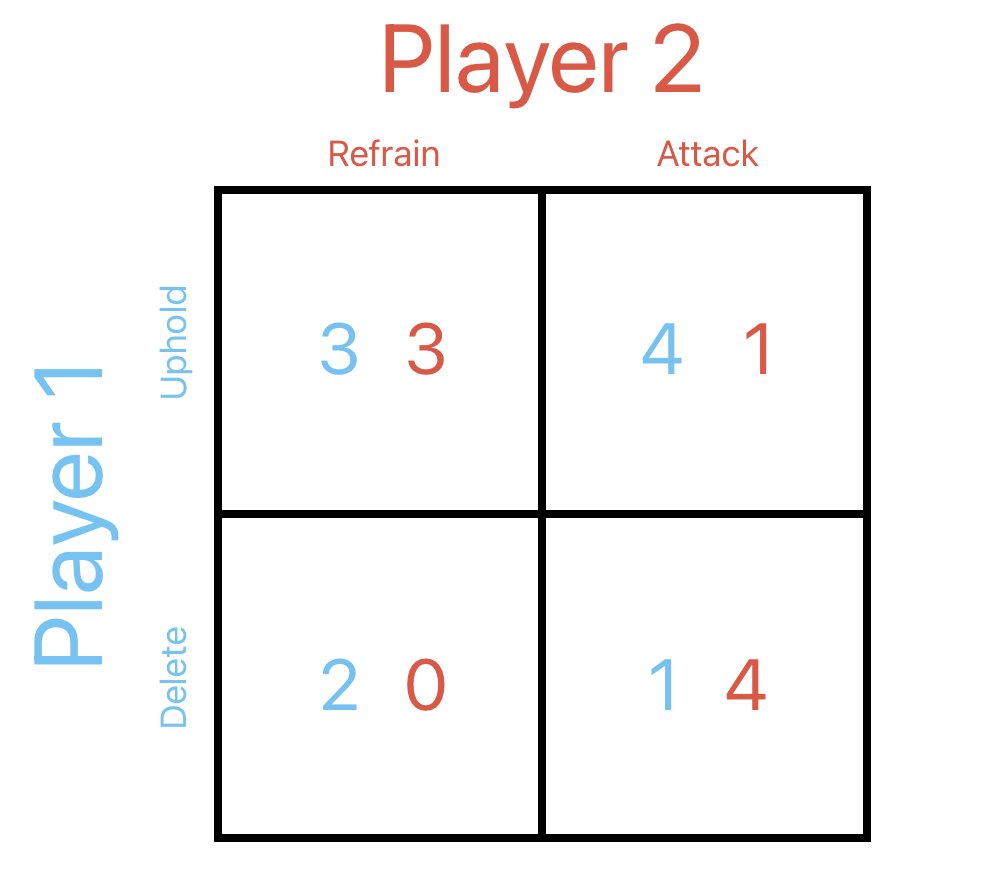
\includegraphics[scale=0.5]{graphics/Player 1.png}
    \caption{Game Theory Table}
    \label{fig:game-theory}
\end{figure}

Seeing this table gives us a payoff for each player based on a certain decision. Using this, we can construct a geometric series from Player 1’s choices below, where delta represents the change over time (think of each delta representing an iteration of the game):

\begin{itemize}
    \item Equilibrium payoff: \[ 3 + 3\Delta + 3\Delta^2 + \dots \]
    \item Defection payoff: \[ 2 + 1\Delta + 1\Delta^2 + 1\Delta^3 + \dots \]
\end{itemize}

The equilibrium payoff remains 3 throughout the course of the geometric series because Player 2 has no choice but to refrain from attacking the subdomain (or otherwise, both players choose to cooperate). For the defection payoff however, Player 1 will receive a payoff of 2 initially, but then receives a payoff of 1 for the remainder of the series due to Player 2 choosing to defect (and thus, both players defect indefinitely). By creating an inequality between these two geometric series, we can calculate the value of delta at which Player 1 should continue the grim trigger strategy, given the condition holds:

\[ 3 + 3\Delta + 3\Delta^2 + \dots \geq 2 + 1\Delta + 1\Delta^2 + 1\Delta^3 + \dots \]

By using some basic algebra, we can reduce this inequality into:

\[ \frac{3}{(1 - \Delta)} \geq 2 + \frac{\Delta}{(1 - \Delta)} \]

If we reduce this further, we can find out at for which value of delta player 1 should continue to uphold this service.

\bigskip
\begin{mdframed}[backgroundcolor=blue!10,style=code,nobreak=true,align=center,userdefinedwidth=14cm]
    \textbf{Action}
    \bigskip
    
    1.2.1 - What is the value of delta at which player 1 continues to uphold?
\end{mdframed}

%%%%%%%%%%%%%%%%%%%%%%%%%%%%%%%%%%%%%%%%%
%%% Task 2
%%%%%%%%%%%%%%%%%%%%%%%%%%%%%%%%%%%%%%%%%

\section*{Task Set 2: Subdomain Takeover}\label{sec:Task Set 2: Subdomain Takeover}
\bigskip
\addcontentsline{toc}{section}{Task Set 2: Subdomain Takeover}

\subsection*{Task 2.1: Attack Surface Enumeration}
\addcontentsline{toc}{subsection}{Task 2.1: Attack Surface Enumeration}

Navigate to the website \url{https://www.geeksforgeeks.org} through your web browser. This domain is a simple static website hosted through Amazon Route 53 and Amazon AWS EC2. This domain works by using an A record to associate the domain name to the IP address within the server. You can access the IP address of this domain by utilizing the dig command within Linux. Open up a new terminal session and run the command \texttt{dig [domain] +short}.

\bigskip
\begin{mdframed}[backgroundcolor=blue!10,style=code,nobreak=true,align=center,userdefinedwidth=14cm]
    \textbf{Action}
    \bigskip
    
    2.1.1 - What is the IP address the DNS server associates with this domain?
\end{mdframed}

Now navigate to the website \url{https://www.maciej.pacut.pl}. This is an example of a subdomain that is utilizing a GitHub service to host a static website. Navigate to the GitHub counterpart, \url{https://www.foo.github.io}. You will see that this service hosts the same content, and thus, is being referenced by the subdomain \url{maciej.pacut.pl}. 

\bigskip
\begin{mdframed}[backgroundcolor=blue!10,style=code,nobreak=true,align=center,userdefinedwidth=14cm]
    \textbf{Action}
    \bigskip
    
    2.1.2 - Based on this information, what record is being resolved in \\Route53 under the subdomain foo.example.com?
\end{mdframed}

Now, within your given project files, open the file domains.txt. This text file serves the list of the primary domain name and all of the subdomains attached to it. Each domain has an active (or inactive) resource associated with it that is resolved by the DNS server Route53. It is up to you to determine what subdomains are vulnerable. Within your project files, you will notice a directory called takeover-py. Navigate into this directory. Within the directory, you will find the README file. Read through the documentation provided within this file. It is important to be able to review open-source projects and understand how to use them. Answer the following questions:

\bigskip
\begin{mdframed}[backgroundcolor=blue!10,style=code,nobreak=true,align=center,userdefinedwidth=14cm]
    \textbf{Action}
    \bigskip
    
     2.1.3 - What is the command you can use to run a DNS enumeration on a text file of domains?\\
     2.1.4 - Run this command on the domains.txt file. This will provide an output of the potentially vulnerable domains and the associated services they use to operate. Submit a screenshot of this output.
\end{mdframed}

Now it is important to decide what subdomain you will attempt to \\takeover/attack. Review the list of services output by the program in the previous step. Each service will have a different approach to hosting and deploying a resource under that name. While each step is easy, you will need to pick one based on your preferences from your understanding of the process involved for each step.

\bigskip
\begin{mdframed}[backgroundcolor=blue!10,style=code,nobreak=true,align=center,userdefinedwidth=14cm]
    \textbf{Action}
    \bigskip
    
    2.1.5 - List the name of the subdomain that you will attack and the service it utilizes.
\end{mdframed}

Now that you have chosen your domain, we can take a few steps to help enumerate the attack surface. In this step, we will utilize the full output of the dig command that we ran in the previous step. This will return a list of the records associated with that subdomain, including an A record reference to the apex zone domain, as well as a CNAME record to a third-party resource.

\bigskip
\begin{mdframed}[backgroundcolor=blue!10,style=code,nobreak=true,align=center,userdefinedwidth=14cm]
    \textbf{Action}
    \bigskip
    
    2.1.6 - Run the command \texttt{dig [domain]} on the specific domain you have been provided. Submit a screenshot of the result.
\end{mdframed}

The output of this file is particularly important to take note of, as it provides key information into how you can takeover the subdomain. For example, it may list the location of the server (na-east), the username of the individual hosting the service (username.github), or even the name of the project (project.surge). All this information depends on the service you chose to use to takeover the subdomain.

\subsection*{Task 2.2: Subdomain Takeover}
\addcontentsline{toc}{subsection}{Task 2.2: Subdomain Takeover}

This section will teach you how to takeover a subdomain through a various service. Refer to the appropriate section below:

\subsubsection*{GitHub}
\addcontentsline{toc}{subsubsection}{GitHub}

This section will teach you how to takeover a GitHub subdomain. The first step is to take note of the information provided from the step performed in the previous section. After running the \texttt{dig [domain]} command, the result will provide you the link of the resource being referenced by the subdomain. This can be in the highlighted section in figure \ref{fig:github-dig}

\begin{figure}[!h]
    \centering
    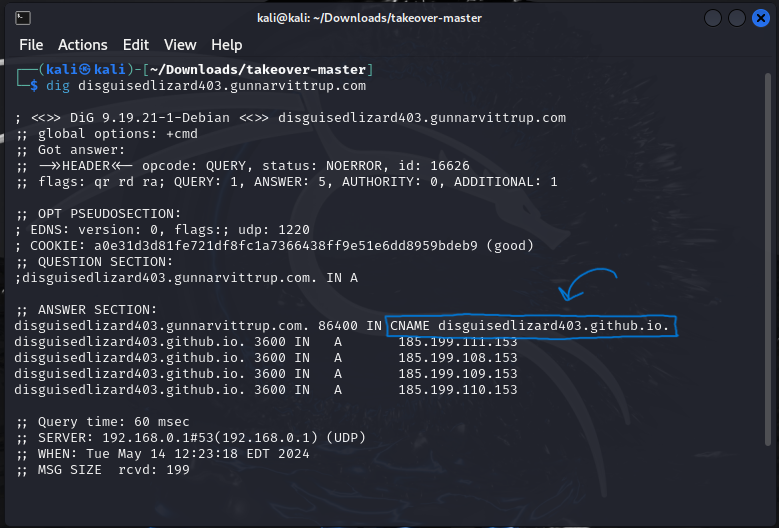
\includegraphics[scale=0.5]{graphics/github dig.png}
    \caption{GitHub Dig}
    \label{fig:github-dig}
\end{figure}

The first bit of the URL following the command specifies the username of the GitHub account that you will need to create in order to take this the subdomain. Head over to GitHub and create a new account using the specified username.

\begin{figure}[!h]
    \centering
    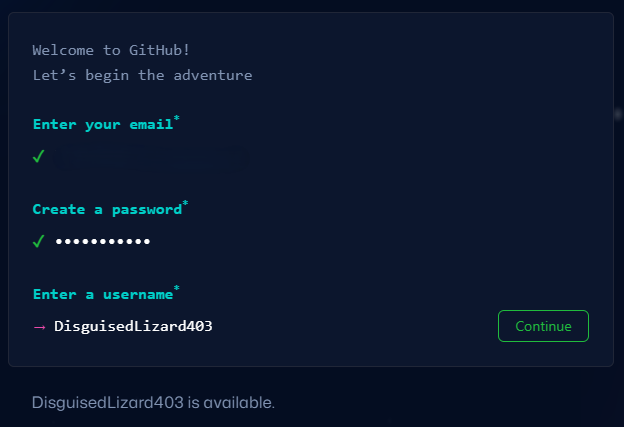
\includegraphics[scale=0.5]{graphics/git create account.png}
    \caption{Creating an Account}
    \label{fig:git-create-account}
\end{figure}

Once you have successfully created an account, you then need to create a repository. The name of this repository needs to be the URL given by the \texttt{dig} command. This is the format for GitHub Pages and is the empty resource being referenced by the subdomain (figure \ref{fig:git-create-repository}).

\begin{figure}[!h]
    \centering
    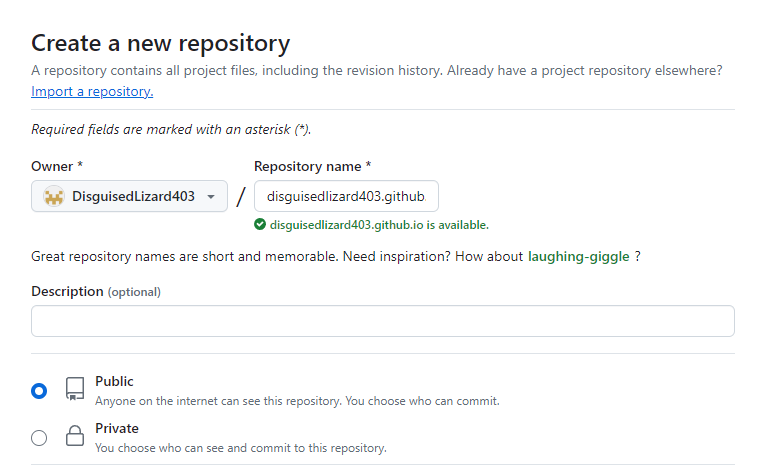
\includegraphics[scale=0.6]{graphics/git create repository.png}
    \caption{Creating a Repository}
    \label{fig:git-create-repository}
\end{figure}

Now that your repository is created, you need to create two files within this repository: an \texttt{index.html} file and a \texttt{CNAME} record. The \texttt{index.html} file (figure \ref{fig:git-index}) will serve as the HTML that is displayed on the subdomain once taken over. The \texttt{CNAME} record (figure \ref{fig:git-cname}) instantiates a DNS check that allows our resource to be referenced by the subdomain, and the content of this file is simply the name of the subdomain URL. 

\begin{figure}[!h]
    \centering
    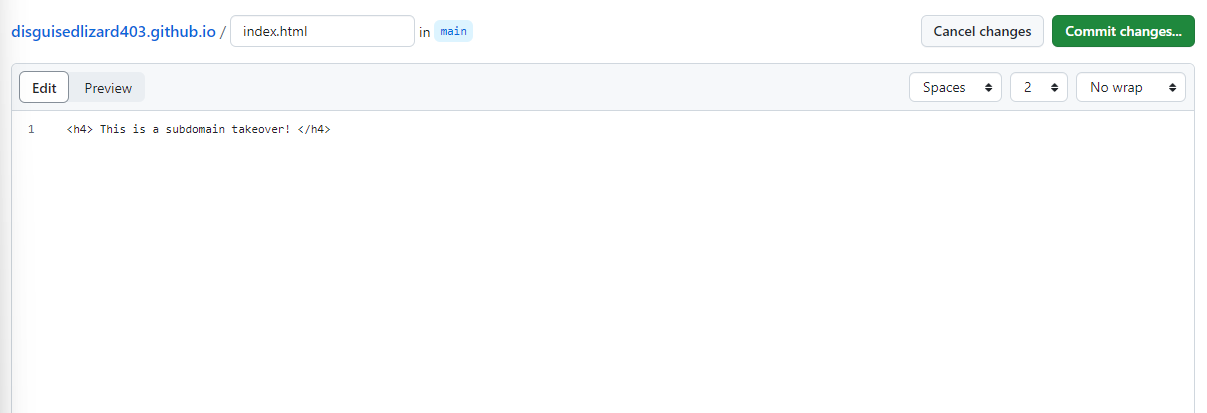
\includegraphics[scale=0.5]{graphics/git index.png}
    \caption{index.html}
    \label{fig:git-index}
\end{figure}

\begin{figure}[!h]
    \centering
    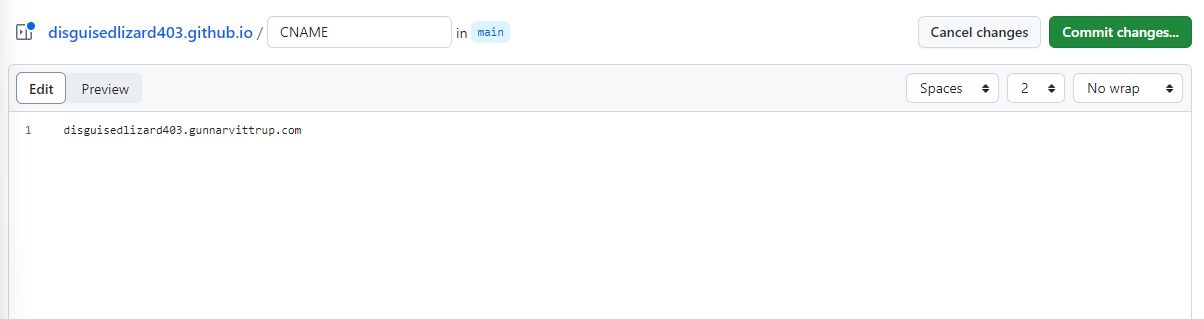
\includegraphics[scale=0.5]{graphics/git cname.png}
    \caption{CNAME}
    \label{fig:git-cname}
\end{figure}

Once these files are created, navigate to the settings of your repository. Under Pages > Custom Domain, you should see that a DNS check is either being performed or is completed on the subdomain specified in your \texttt{CNAME} record. Once this check has been completed successfully, you should be able to navigate to the original subdomain and see the content of your \texttt{index.html} file being displayed. This concludes a successful subdomain takeover attack using GitHub as a service. 

\begin{figure}[!h]
    \centering
    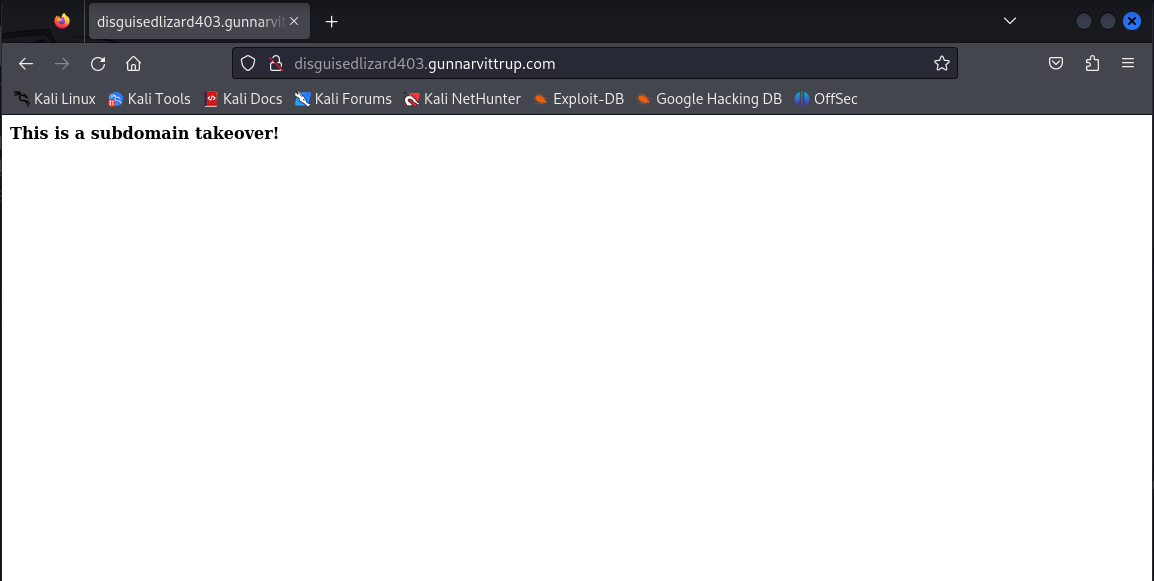
\includegraphics[scale=0.5]{graphics/git takeover.png}
    \caption{Successful GitHub Takeover}
    \label{fig:git-takeover}
\end{figure}

\subsubsection*{Surge}
\addcontentsline{toc}{subsubsection}{Surge}

This section will teach you how to takeover a Surge subdomain. The first step is to take note of the information provided from the step performed in the previous section. After running the \texttt{dig [domain]} command, the result will provide you the link of the resource being referenced by the subdomain. This can be in the highlighted section in figure \ref{fig:surge-dig}

\begin{figure}[!h]
    \centering
    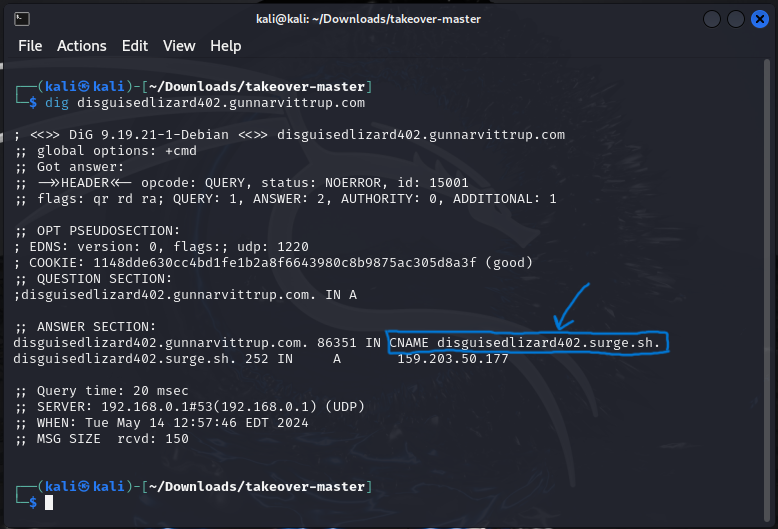
\includegraphics[scale=0.45]{graphics/surge dig.png}
    \caption{Surge Dig}
    \label{fig:surge-dig}
\end{figure}

To start, open a new terminal window. We need to install a few different services that will allow us to utilize Surge to host a website. Run the steps below in the order given:

\bigskip
\begin{enumerate}
    \item \texttt{sudo apt install npm}
    \item \texttt{npm install -{}-global node}
    \item \texttt{npm install -{}-global surge}
\end{enumerate}

NPM is a package manager that provides access to various JavaScript programs and software, Node is a server-side scripting framework, and Surge is a cloud platform for hosting websites. With these tools alone, we can successfully take over a given subdomain utilizing Surge as a service. Create a new directory using the \texttt{mkdir} command and use the \texttt{cd} command to move into it. Within this directory, create two new files using the \texttt{nano} command: an \texttt{index.html} file and a \texttt{CNAME} record. The index.html file (figure \ref{fig:surge-index}) will serve as the HTML that is displayed on the subdomain once taken over. The CNAME record (figure \ref{fig:surge-cname}) instantiates a DNS check that allows our resource to be referenced by the subdomain, and the content of this file is simply the name of the subdomain URL.

\begin{figure}[!h]
    \centering
    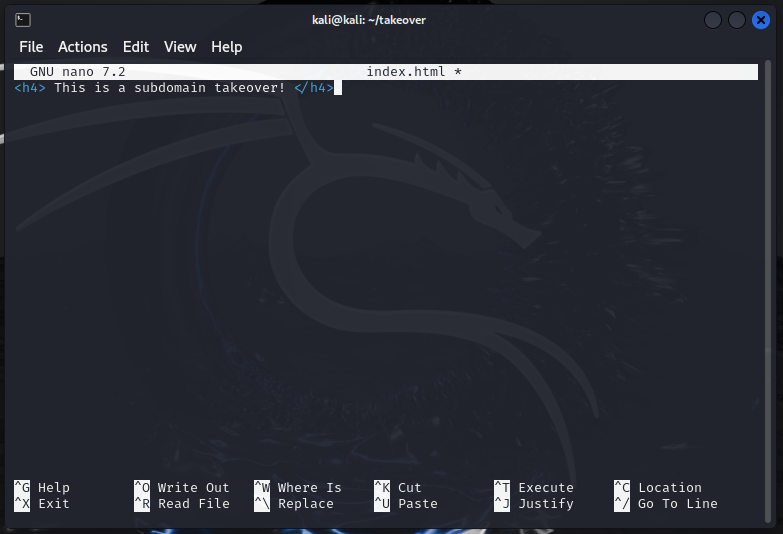
\includegraphics[scale=0.45]{graphics/surge index.png}
    \caption{index.html}
    \label{fig:surge-index}
\end{figure}

\begin{figure}[!h]
    \centering
    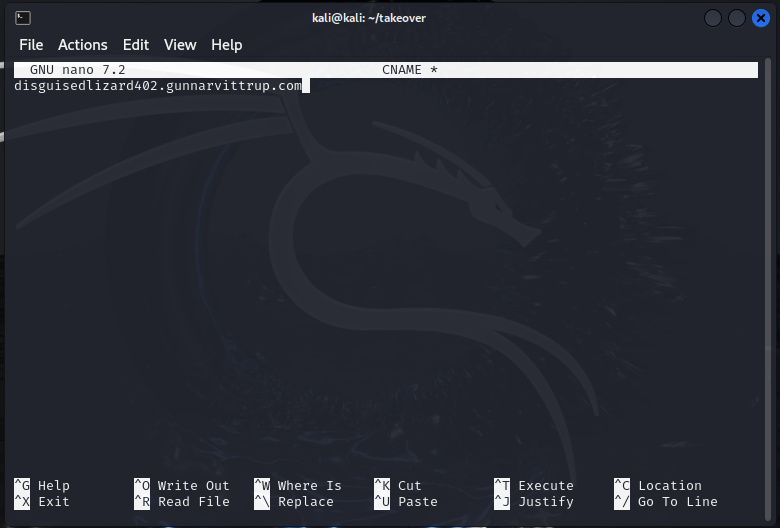
\includegraphics[scale=0.45]{graphics/surge cname.png}
    \caption{CNAME}
    \label{fig:surge-cname}
\end{figure}

Once these two files have been created, now it is time to make use of our newly installed \texttt{Surge} package. While inside of the newly-created directory, run the command \texttt{surge} to deploy it. 

\begin{figure}[!h]
    \centering
    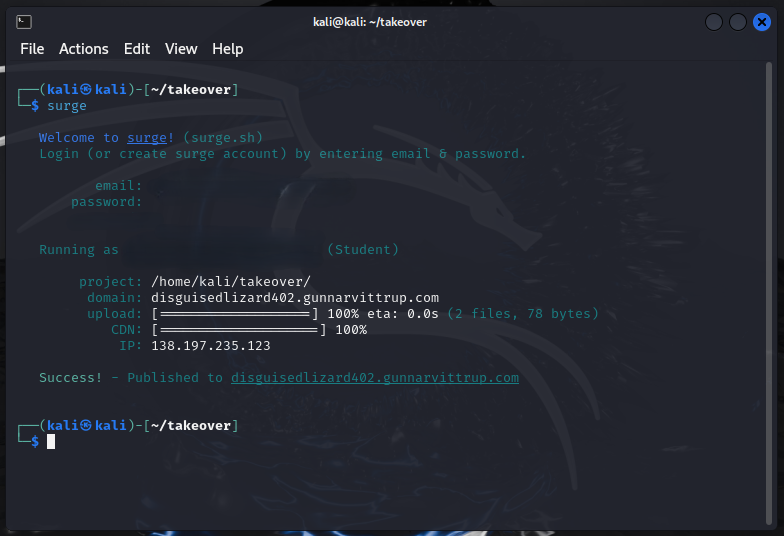
\includegraphics[scale=0.45]{graphics/run surge.png}
    \caption{Running Surge}
    \label{fig:run-surge}
\end{figure}

Once you have successfully iterated through all of the prompts given by this command, verify that your deployment and takeover has been successful by navigating to the original subdomain. 

\begin{figure}[!h]
    \centering
    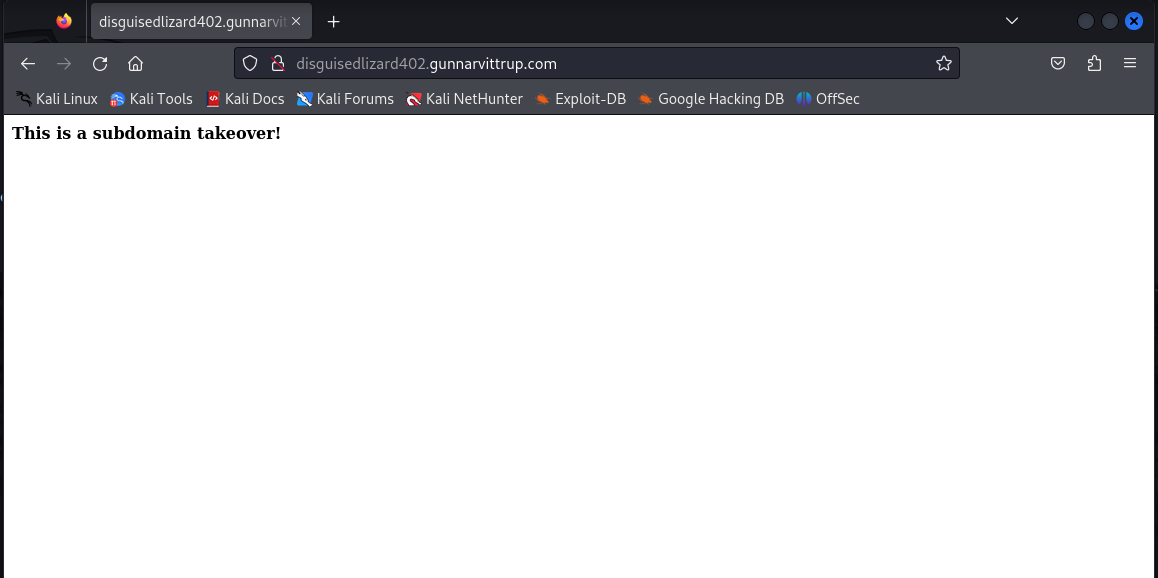
\includegraphics[scale=0.5]{graphics/surge takeover.png}
    \caption{Successful Surge Takeover}
    \label{fig:surge-takeover}
\end{figure}

\bigskip
\begin{mdframed}[backgroundcolor=blue!10,style=code,nobreak=true,align=center,userdefinedwidth=14cm]
    \textbf{Action}
    \bigskip
    
    2.2.1 - Take over the subdomain listed in your previous answer and submit a screenshot of the page displaying the content within your index.html file.
\end{mdframed}

After finishing the previous section, it is important to release any empty resources that you created for the purpose of this lab. 

%%%%%%%%%%%%%%%%%%%%%%%%%%%%%%%%%%%%%%%%%
%%% Submission
%%%%%%%%%%%%%%%%%%%%%%%%%%%%%%%%%%%%%%%%%

\section*{Submission}\label{sec:Submission}
\addcontentsline{toc}{section}{Submission}

Submit a lab report utilizing the provided template to your instructor, which should include screenshots, thoughts, challenges, and lessons learned from the lab.

%%%%%%%%%%%%%%%%%%%%%%%%%%%%%%%%%%%%%%%%%
%%% Summary
%%%%%%%%%%%%%%%%%%%%%%%%%%%%%%%%%%%%%%%%%

\section*{Summary}\label{sec:Summary}
\addcontentsline{toc}{section}{Summary}

Many websites and web applications make use of third-party services/resources to host static or dynamic sites for a myriad of different reasons. Without proper steps or protocol, these services and resources can lead to weak points within a domain, all while being incredibly easy to enumerate. Our focus in this lab was to recognize, enumerate, and abuse these vulnerabilities in order to take control over a sibling domain. By performing a proof of concept attack, we further explore conventional security protocols that can prevent these attacks. 

\bibliography{References}
\bibliographystyle{plain}

\end{document}

%%%%%%%%%%%%%%%%%%%%%%%%%%%%%%%%%%%%%%%%%